\chapter{And One More Chapter}\label{ch:z}

Ignatius is something of a modern Don Quixote --- eccentric, idealistic, and creative, sometimes to the point of delusion. In his foreword to the book, Walker Percy describes Ignatius as a slob extraordinary, a mad Oliver Hardy, a fat Don Quixote, a perverse Thomas Aquinas rolled into one. He disdains modernity, particularly pop culture. The disdain becomes his obsession: he goes to movies in order to mock their perversity and express his outrage with the contemporary world's lack of theology and geometry. He prefers the scholastic philosophy of the Middle Ages, and the Early Medieval philosopher Boethius in particular. However he also enjoys many modern comforts and conveniences, and is given to claiming that the rednecks of rural Louisiana hate all modern technology which they associate with progress.

\section{an intro section}\label{sec:z1}

Si $f(x)= 45$ entonce\ldots.

Introduccionasd \ref{fig:santa-fe}as


\begin{figure}[t]
\centering
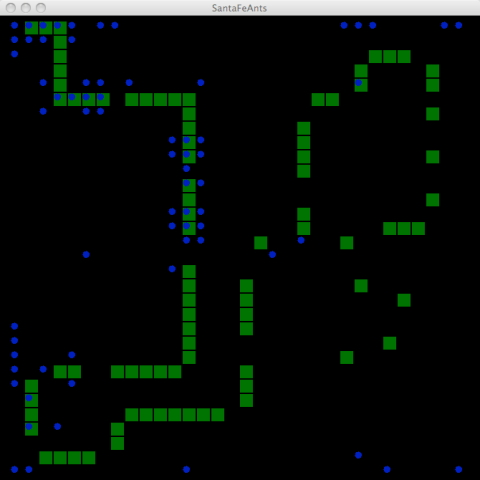
\includegraphics[width=0.65\textwidth]{figs/santa-fe-trail}
\caption{Representación del problema del camino de la hormiga de Santa Fe.}
\label{fig:santa-fe}
\end{figure}


\begin{table}[tb]
\caption{Mi tablita linda.}
\label{tab:comparison}
\centering
\begin{tabular}{lccc}
\toprule
\textbf{MOEA} & \textbf{MGBM} & \textbf{\citet{deb-thiele-laumanns-zitzler-04:scalable-test-problems}} & \textbf{\citet{Khare02}}\\
\otoprule
\multicolumn{4}{c}{\textbf{DTLZ3}}\\
\midrule
NSGA--II &  $91$, $104$, $115$ & $500$ & $500$ \\
SPEA2    & $121$, $132$, $149$ & $500$ & $500$ \\
PESA     & $125$, $129$, $138$ & $500$ & $500$ \\
\midrule
\multicolumn{4}{c}{\textbf{DTLZ6}}\\
\midrule
NSGA--II & $104$, $106$, $140$ & $500$ & $500$ \\
SPEA2    &  $71$,  $78$, $123$ & $500$ & $500$ \\
PESA     &  $95$, $103$, $151$ & $500$ & $500$ \\
\midrule
\multicolumn{4}{c}{\textbf{DTLZ7}}\\
\midrule
NSGA--II & $237$, $259$, $275$ & $200$ & --- \\
SPEA2    & $269$, $305$, $330$ & $200$ & --- \\
PESA     & $279$, $298$, $326$ & $200$ & --- \\
\bottomrule
\end{tabular}
\end{table}

\begin{equation}
   fitness = \sum_{i}w_if_i(x),
\end{equation}
donde $f_i(x)$ es el valor obtenido al evaluar la $i$-ésima función objetivo y  $w_i$ el valor por el cual
misma se poderará.